\label{sec:discussion:subsec:convergence}
\begin{figure}[t]
     \subfloat[][Workflow net mined from the log of Pharmaceutical company.]{
\includegraphics[width=0.37\linewidth]{content/figures/pharma_dep1.pdf}\label{fig:wfnet:a}}
     \hfill
     \subfloat[][Workflow net mined from the log of Specialized clinic.]{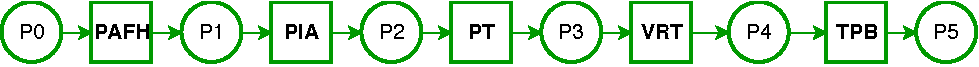
\includegraphics[width=0.57\linewidth]{content/figures/specialised_dep1.pdf}\label{fig:wfnet:b}}
      \hfill
      \vspace{1em}
     \subfloat[][Workflow net mined from the log of Hospital.]{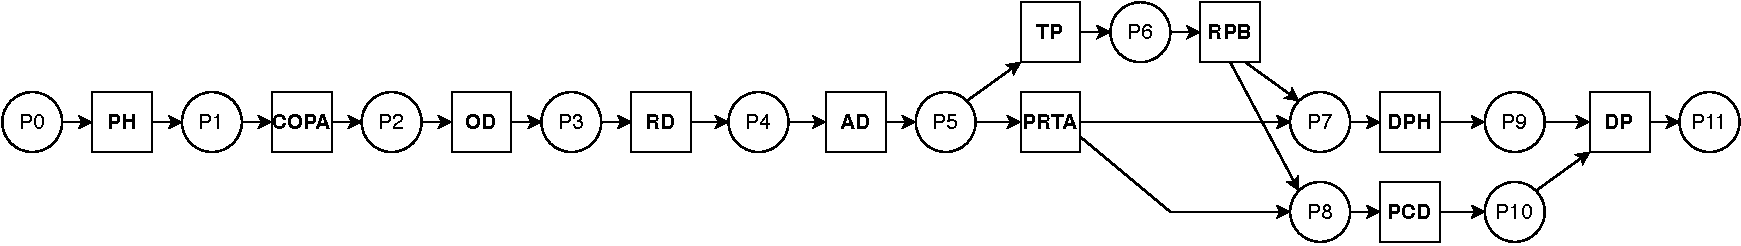
\includegraphics[width=1\linewidth]{content/figures/hospital_dep1.pdf}\label{fig:wfnet:c}}
      \hfill
      \vspace{1em}
      \subfloat[][Workflow net mined from the merged log in inter-organizational setting.]{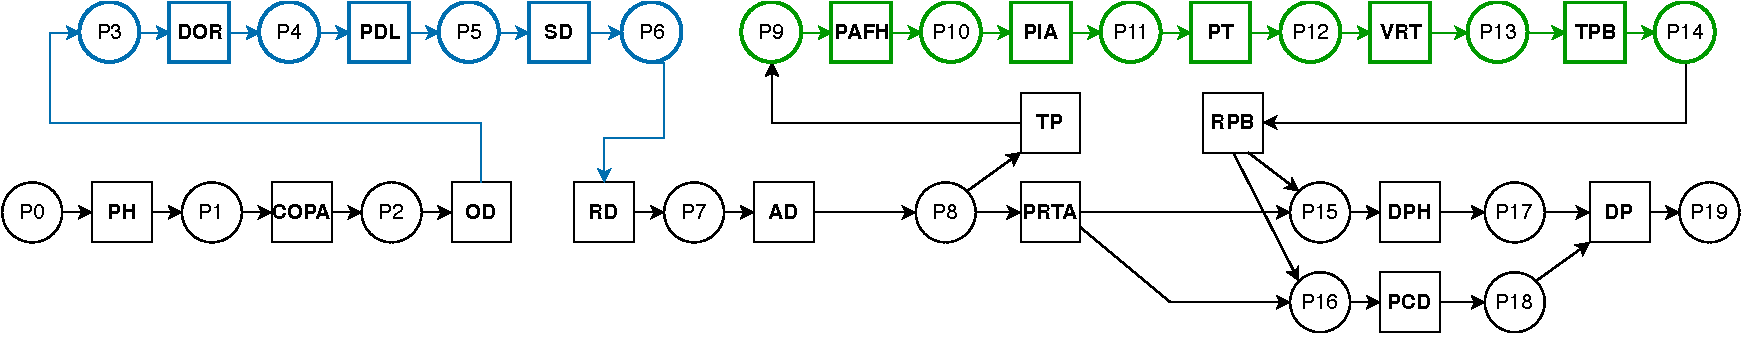
\includegraphics[width=1\linewidth]{content/figures/merged_dep1.pdf}\label{fig:wfnet:d}}
     \caption{Outputs used for the convergence test.}
     \label{fig:wfnet}
\end{figure}
\section{Discussion}
\label{sec:evaluation}

\begin{comment}
\todo[inline]{CDC: MISSING:
Nella evaluation, dobbiamo riportare l'uso di memoria qui conta perché è un parametro fondamentale.
\\
Dobbiamo informare il lettore sulle caratteristiche del log (numero eventi, numero tracce, dimensione totale in KB una volta salvato in formato XES), come lo abbiamo creato, perché il modello non è uguale a quello di Fig. 1.}
\end{comment}


In this section, we evaluate the proposed approach. The primary objective of the \cref{sec:discussion:subsec:convergence} is to delve into a convergence analysis by evaluating the efficacy of the collaborative data exchange process. We then took into assessment the memory usage by measuring the RAM usage in diverse parameter configurations in \cref{sec:discussion:subsec:memory}. In \cref{sec:discussion:subsec:validation}, we validate the addressed approach using real-world data to conclude the discussion. 

\subsection{Datasets}
\todo[inline]{the following text was in the implementation and was moved here }
In order to generate the logs for the execution of the trusted application, we produced a simulation model based on our running example (see~\cref{sec:motivating}).% was created based on BPMN notation\footnote{https://www.bpmn.org}. Subsequently, the model was imported fed as input into the BIMP tool.%
\footnote{https://bimp.cs.ut.ee}
% which made it possible to generate the synthetic event logs. 
The number of log traces generated through BIMP aligns with other works in the state of the art; the generation software was set to 1000 traces.
\todo{Mention Sepsis here}
Following the generation, the synthetic event log relating to the process model was filtered via ProM.%
\footnote{https://promtools.org}
We were able to filter the logs based on attribute values, which allowed us to filter the synthetic log according to the resource involved in the activities. Referring to the motivating scenario, the resources involved are the hospital, the specialized clinic, and the pharmaceutical company. In this way, we created three separate event logs from the initial event log, which were used to exchange data between the organizations.


\subsection{Convergence}
\label{sec:discussion:subsec:convergence}  
%\todo[inline]{Dobbiamo informare il lettore sulle caratteristiche del log (numero eventi, numero tracce, dimensione totale in KB una volta salvato in formato XES), come lo abbiamo creato, perché il modello non è uguale a quello di Fig. 1.}

We take into analysis the convergence of the process discovery outputs, as a way of validating the correct operation of the event log exchange mechanism, . Specifically, we generated the workflow nets computed in an intra-organizational setting, in which each organization directly mines its own event log. Subsequently, we employed our approach with a miner actor that computes the same discovery algorithm using an inter-organizational event log obtained as a result of the log exchange and the merging mechanisms. 

To run the test, we used the synthetic event logs devised from our motivating scenario whose BPMN is depicted in \cref{fig:BPMN_Healthcare}. The size of the \texttt{Hospital}, \texttt{Specialized clinic}, and \texttt{Pharmaceutical company} event logs are 4.8 MB, 1.1 MB, and 1.6 MB respectively.  Each log contains the standard value of 1000 traces, in accordance with the Sepsis Cases \cite{sepsis} event log. %and BPIC 2015 \cite{bpic2015} event logs. % meglio non correre rischi.
% In our experiments, we set the \texttt{Hospital} as the miner.

Upon visual examination of \cref{fig:wfnet}, we observe that the workflow net computed through our approach, displayed in \cref{fig:wfnet:d}, encapsulates the structure and behavior of the workflow nets derived from the intra-organizational discovery procedures depicted in \cref{fig:wfnet:a},\cref{fig:wfnet:b}, and \cref{fig:wfnet:c}. % Transitions and places within both workflow nets exhibit a clear congruence, indicative of a shared underlying process model. 
In detail, \cref{fig:wfnet:a}, colored in blue, depicts the process of the \texttt{pharmaceutical company} from the moment the drug order is received to its fulfillment. \Cref{fig:wfnet:b}, colored in green, depicts the process of the \texttt{Specialized clinic} from the moment the patient arrives from the \texttt{Hospital} to his transfer.
%This congruence further extends to the temporal sequencing of events and the causal relationships among process steps. This substantial resemblance between the two Workflow Nets serves as a testament to the seamless convergence of disparate event logs, achieved through the secure exchange mechanism. The fact that the collaborative process model, represented by the Workflow Net generated from the merged event log, aligns closely with the independent models of individual organizations underscores the fidelity and accuracy of the data exchange process.
% We point out that there are some minor changes between the process model behind the logs used for the tests and the BPMN in \cref{fig:BPMN_Healthcare}. To generate a log that allows us to simulate an inter-organizational scenario, it is necessary to make some simplifications to the presented BPMN syntax. Hence, we explain the slight inconsistencies between the process depicted in the motivating scenario and the process drawn by the workflow net of the test.



\subsection{Memory Usage}
\todo[inline]{grafici memory usage: segment size, }
\label{sec:discussion:subsec:memory}

\begin{figure}[t]
\centering
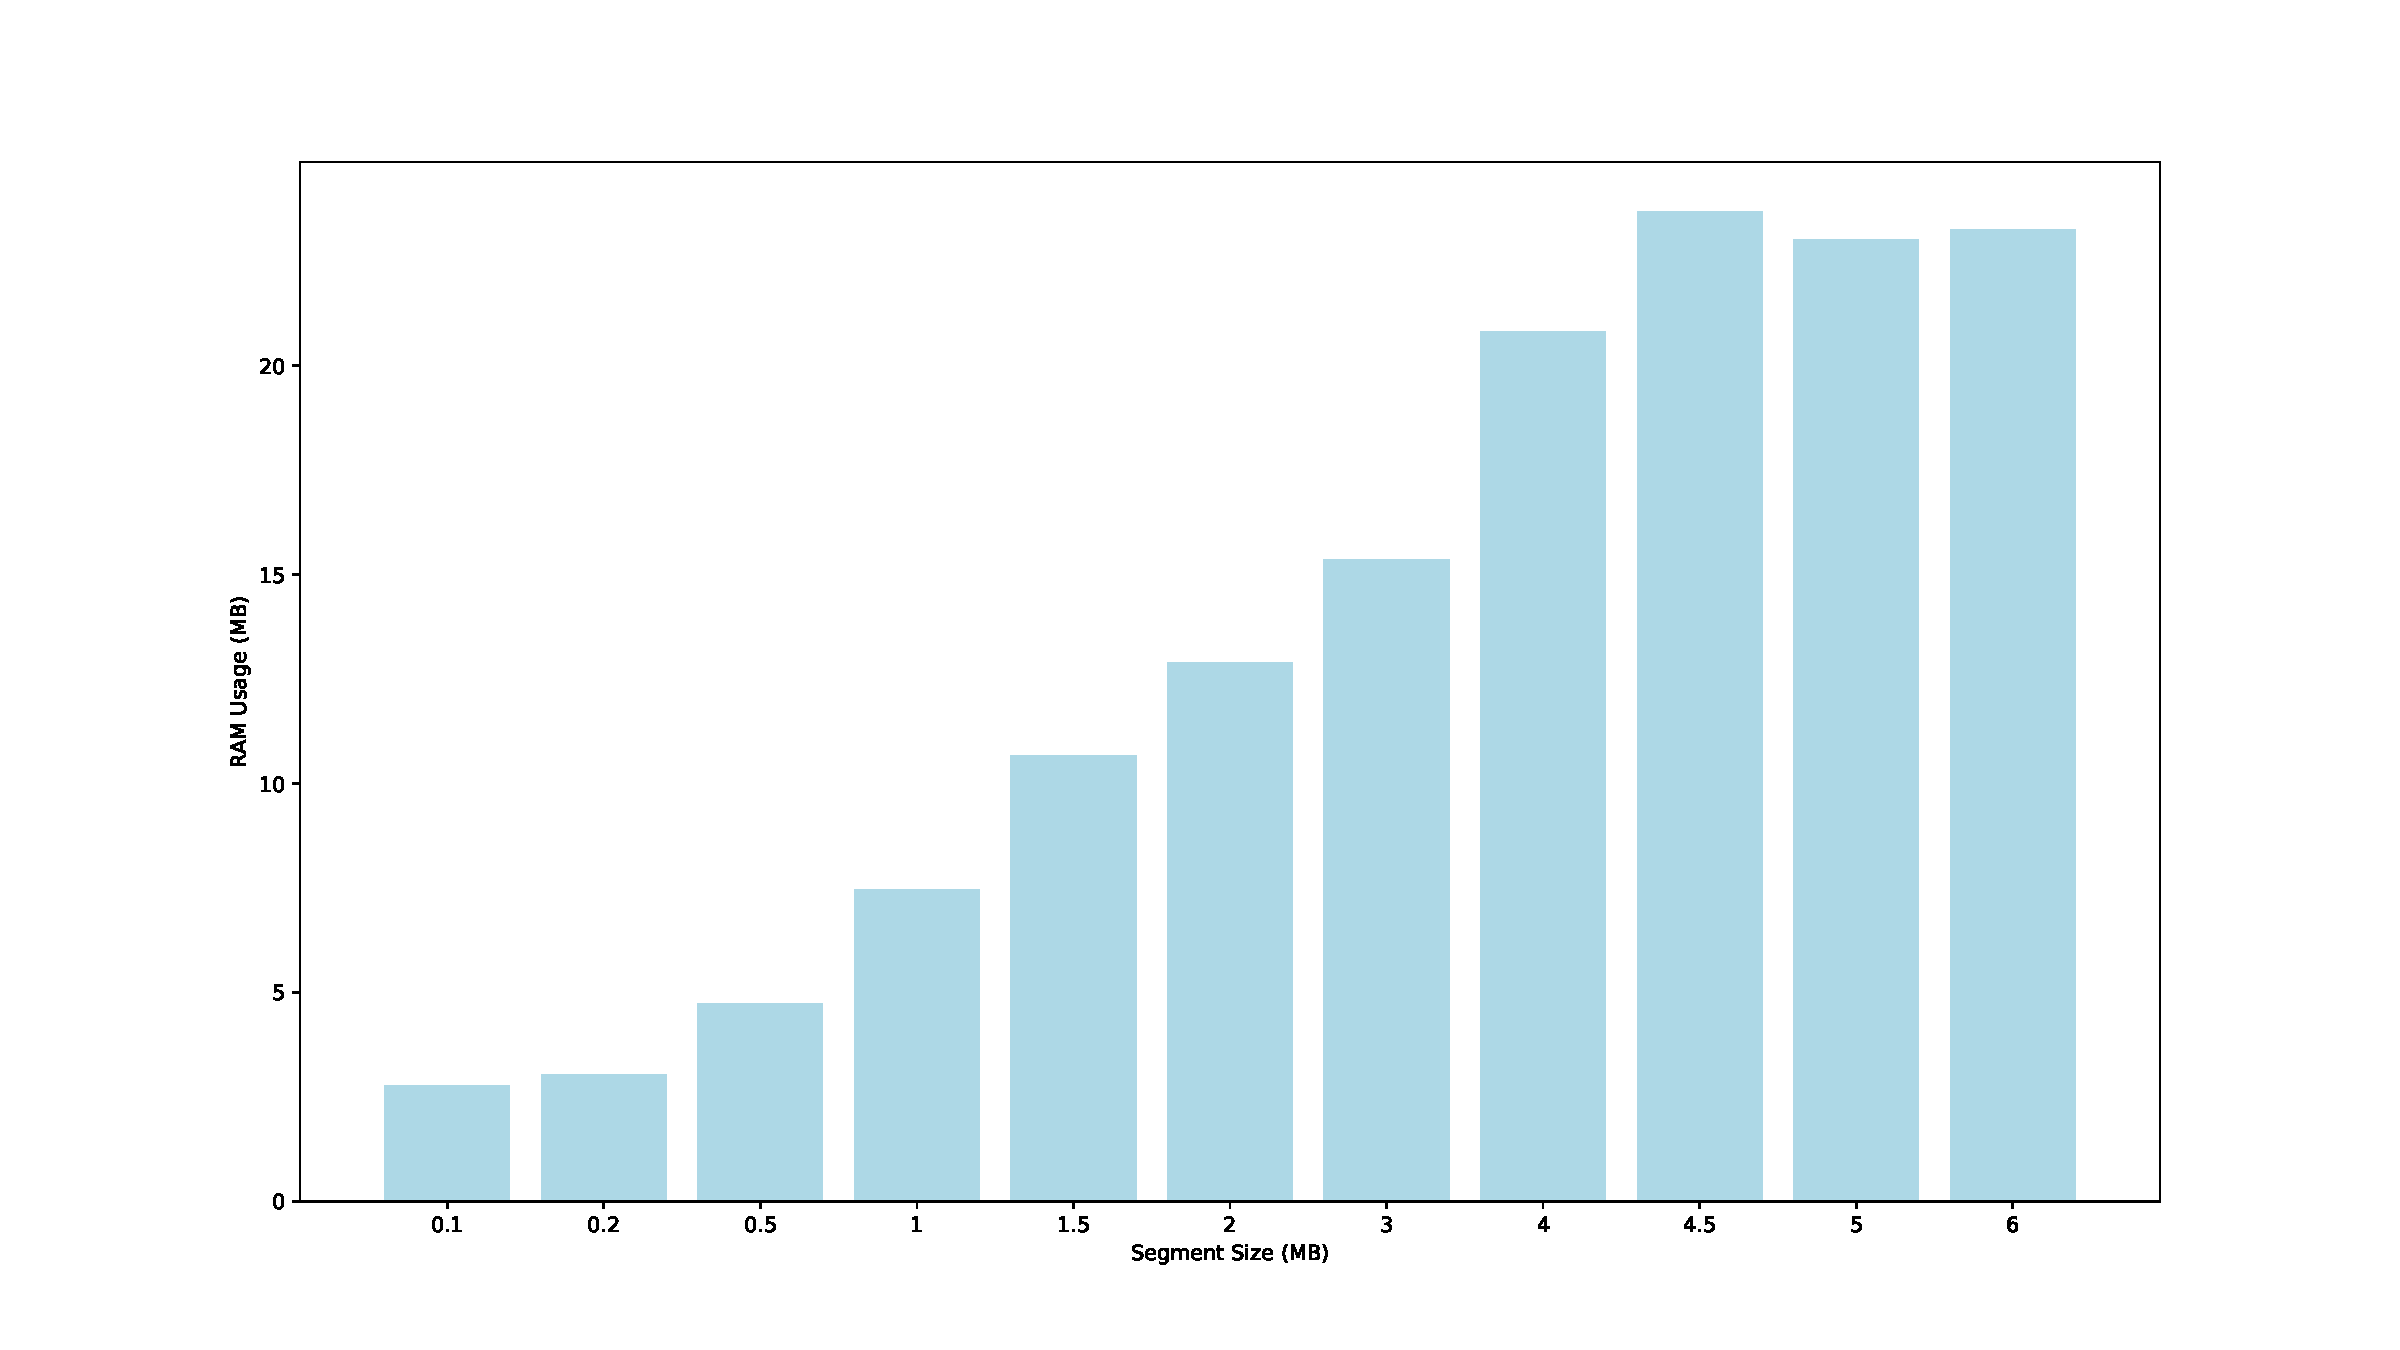
\includegraphics[width=1\linewidth]{content/figures/barplot_segsize.pdf}
\caption{RAM Memory usage for the healthcare synthetic log with 1000 traces}
\label{fig:barplot_segsize}
\end{figure}


\begin{figure}[t]
\centering
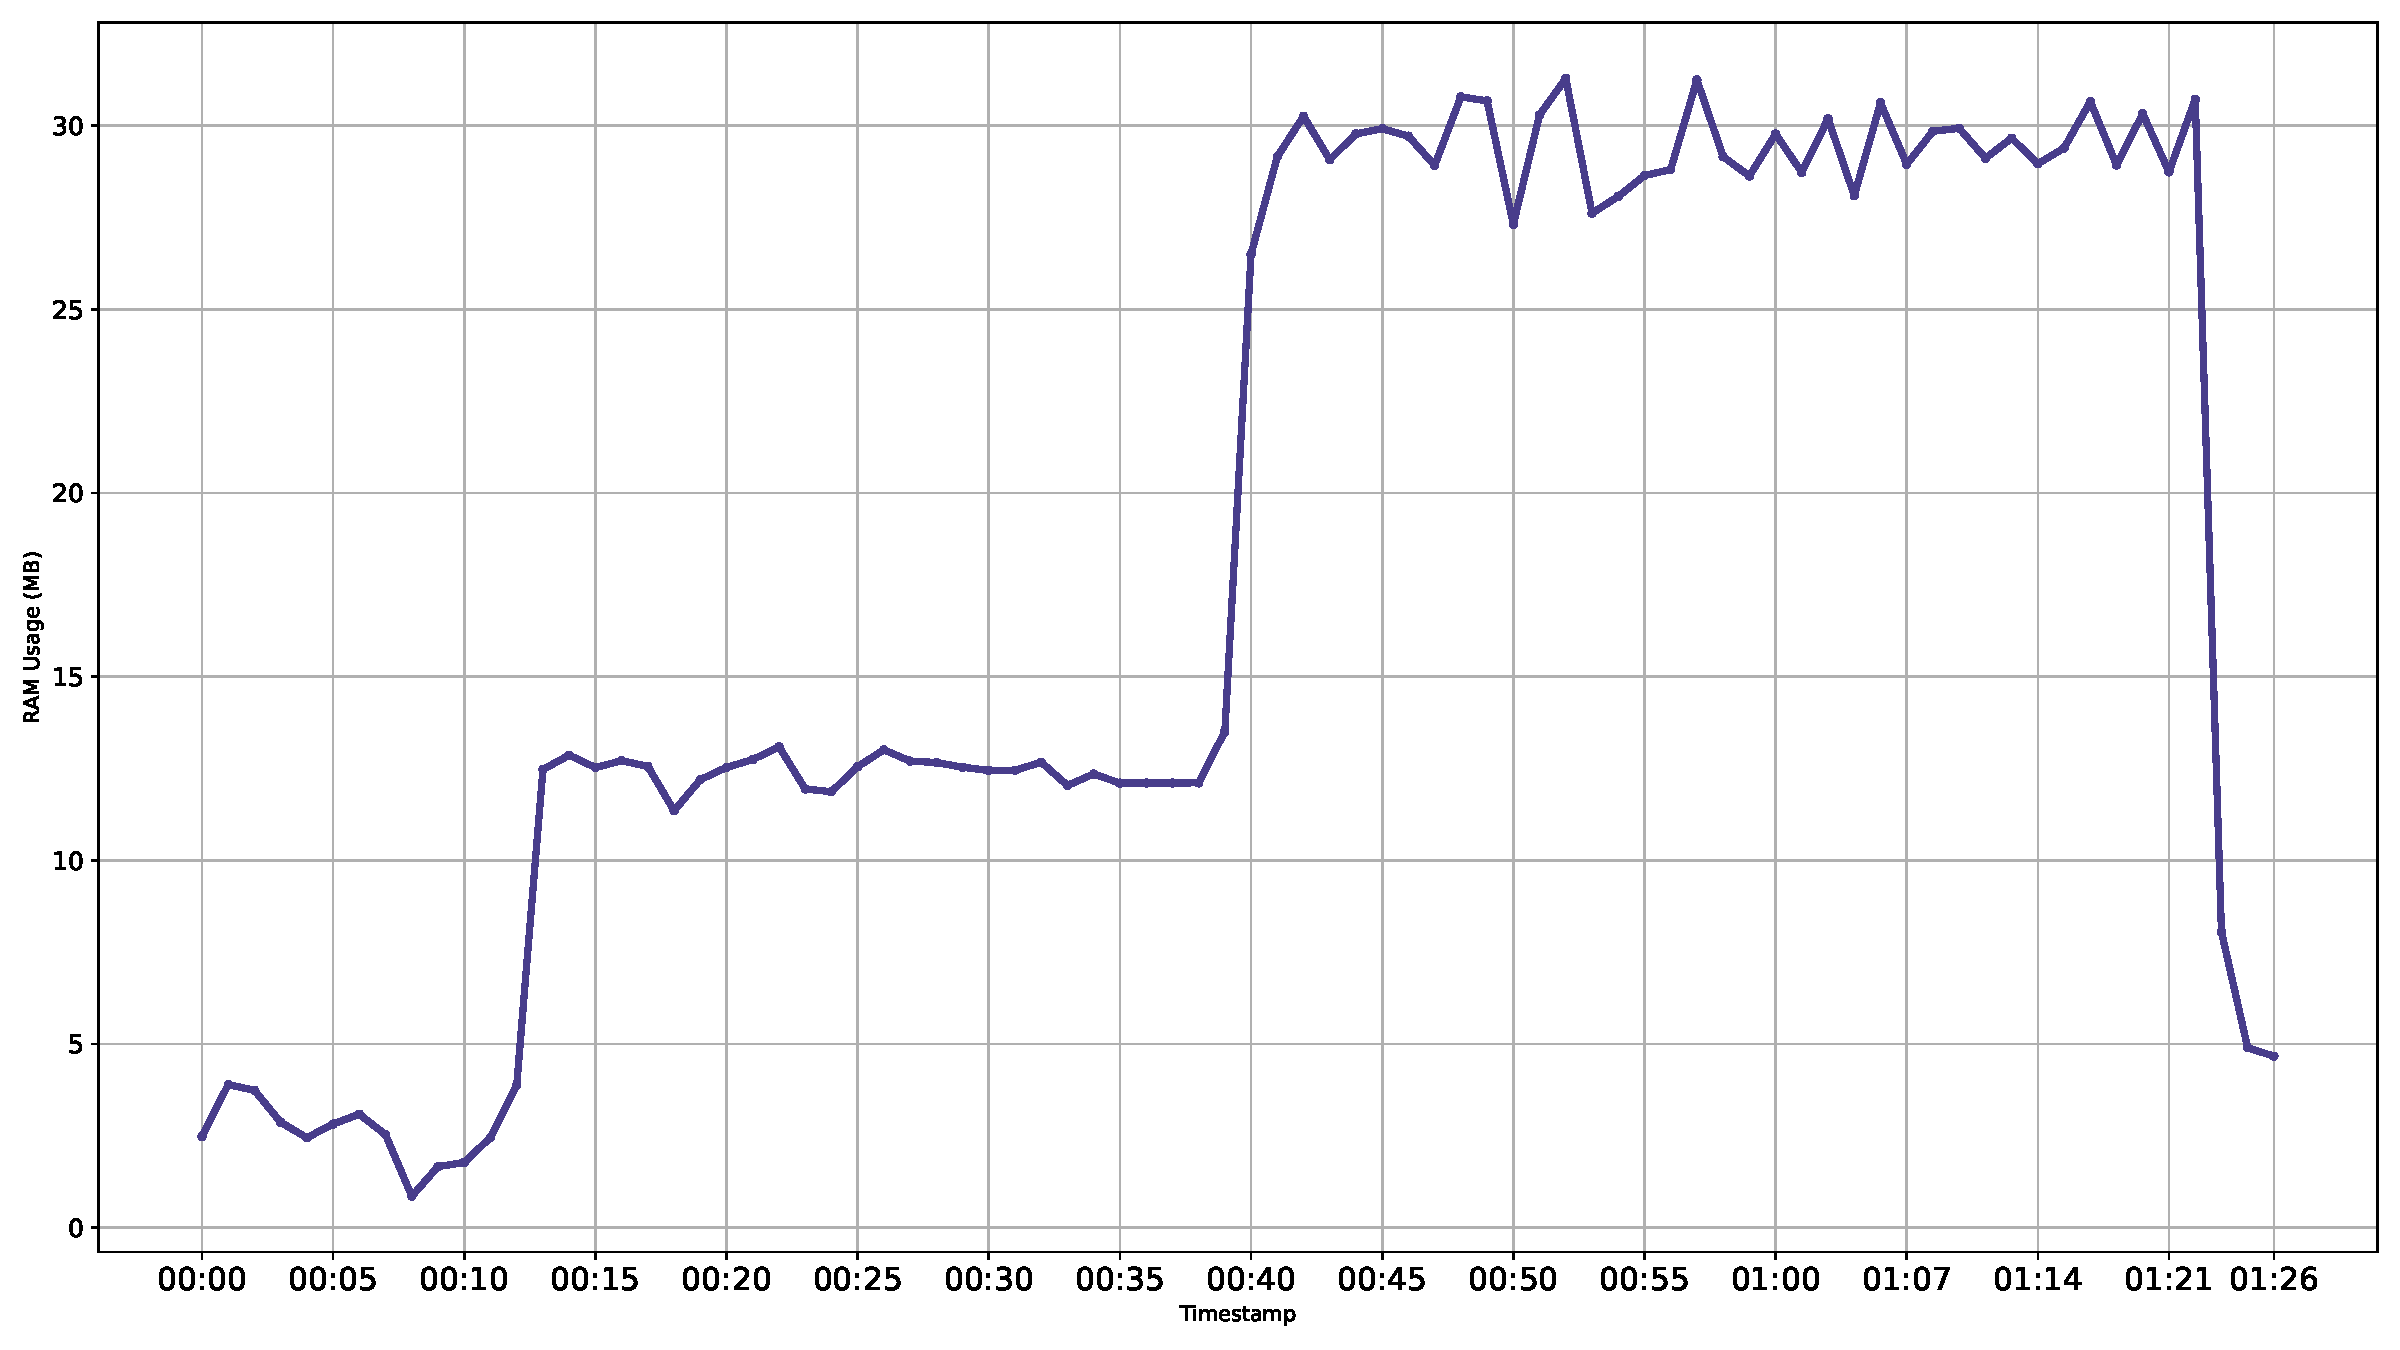
\includegraphics[width=1\linewidth]{content/figures/ram_usage_per_TS.pdf}
\caption{RAM Memory usage for a single run for the healthcare synthetic log with 1000 traces}
\label{fig:ramusage_ts}
\end{figure}

\begin{comment}
\subsection{Integrity and Confidentiality}
\label{sec:discussion:subsec:integrityandconfidentiality}
An essential aspect of the evaluation pertains to the fundamental principles of integrity and confidentiality upheld by the Trusted Execution Environment (TEE), crucial pillars that underpin the effectiveness and trustworthiness of the event log sharing mechanism. In this framework, the TEE is the cornerstone of data processing, demonstrating praiseworthy abilities to ensure data integrity. Throughout the entire process, from the moment data is ingested from individual organizations to the merging of event logs, the TEE maintains an unyielding grip on data integrity, steadfastly safeguarding against unauthorized modifications. This veracity is established through cryptographic hashing and secure storage mechanisms that ensure that the merged event log remains unaltered and representative of the original data. Concurrent with data integrity, the TEE exercises a robust commitment to confidentiality. The cryptographic measures implemented within the TEE ensure that all data, whether in transit or at rest, is encrypted with a level of security that mitigates the risk of unauthorized access. This cryptographic fortification guarantees that sensitive information encapsulated within event logs remains comprehensively shielded, rendering them inaccessible to any unauthorized entities. As a result, participating organizations can confidently share their event logs, knowing that their proprietary and sensitive information remains impervious to prying eyes.
\end{comment}

